% Options for packages loaded elsewhere
\PassOptionsToPackage{unicode}{hyperref}
\PassOptionsToPackage{hyphens}{url}
\PassOptionsToPackage{dvipsnames,svgnames,x11names}{xcolor}
%
\documentclass[
  letterpaper,
  DIV=11,
  numbers=noendperiod]{scrreprt}

\usepackage{amsmath,amssymb}
\usepackage{iftex}
\ifPDFTeX
  \usepackage[T1]{fontenc}
  \usepackage[utf8]{inputenc}
  \usepackage{textcomp} % provide euro and other symbols
\else % if luatex or xetex
  \usepackage{unicode-math}
  \defaultfontfeatures{Scale=MatchLowercase}
  \defaultfontfeatures[\rmfamily]{Ligatures=TeX,Scale=1}
\fi
\usepackage{lmodern}
\ifPDFTeX\else  
    % xetex/luatex font selection
\fi
% Use upquote if available, for straight quotes in verbatim environments
\IfFileExists{upquote.sty}{\usepackage{upquote}}{}
\IfFileExists{microtype.sty}{% use microtype if available
  \usepackage[]{microtype}
  \UseMicrotypeSet[protrusion]{basicmath} % disable protrusion for tt fonts
}{}
\makeatletter
\@ifundefined{KOMAClassName}{% if non-KOMA class
  \IfFileExists{parskip.sty}{%
    \usepackage{parskip}
  }{% else
    \setlength{\parindent}{0pt}
    \setlength{\parskip}{6pt plus 2pt minus 1pt}}
}{% if KOMA class
  \KOMAoptions{parskip=half}}
\makeatother
\usepackage{xcolor}
\setlength{\emergencystretch}{3em} % prevent overfull lines
\setcounter{secnumdepth}{5}
% Make \paragraph and \subparagraph free-standing
\ifx\paragraph\undefined\else
  \let\oldparagraph\paragraph
  \renewcommand{\paragraph}[1]{\oldparagraph{#1}\mbox{}}
\fi
\ifx\subparagraph\undefined\else
  \let\oldsubparagraph\subparagraph
  \renewcommand{\subparagraph}[1]{\oldsubparagraph{#1}\mbox{}}
\fi


\providecommand{\tightlist}{%
  \setlength{\itemsep}{0pt}\setlength{\parskip}{0pt}}\usepackage{longtable,booktabs,array}
\usepackage{calc} % for calculating minipage widths
% Correct order of tables after \paragraph or \subparagraph
\usepackage{etoolbox}
\makeatletter
\patchcmd\longtable{\par}{\if@noskipsec\mbox{}\fi\par}{}{}
\makeatother
% Allow footnotes in longtable head/foot
\IfFileExists{footnotehyper.sty}{\usepackage{footnotehyper}}{\usepackage{footnote}}
\makesavenoteenv{longtable}
\usepackage{graphicx}
\makeatletter
\def\maxwidth{\ifdim\Gin@nat@width>\linewidth\linewidth\else\Gin@nat@width\fi}
\def\maxheight{\ifdim\Gin@nat@height>\textheight\textheight\else\Gin@nat@height\fi}
\makeatother
% Scale images if necessary, so that they will not overflow the page
% margins by default, and it is still possible to overwrite the defaults
% using explicit options in \includegraphics[width, height, ...]{}
\setkeys{Gin}{width=\maxwidth,height=\maxheight,keepaspectratio}
% Set default figure placement to htbp
\makeatletter
\def\fps@figure{htbp}
\makeatother
\newlength{\cslhangindent}
\setlength{\cslhangindent}{1.5em}
\newlength{\csllabelwidth}
\setlength{\csllabelwidth}{3em}
\newlength{\cslentryspacingunit} % times entry-spacing
\setlength{\cslentryspacingunit}{\parskip}
\newenvironment{CSLReferences}[2] % #1 hanging-ident, #2 entry spacing
 {% don't indent paragraphs
  \setlength{\parindent}{0pt}
  % turn on hanging indent if param 1 is 1
  \ifodd #1
  \let\oldpar\par
  \def\par{\hangindent=\cslhangindent\oldpar}
  \fi
  % set entry spacing
  \setlength{\parskip}{#2\cslentryspacingunit}
 }%
 {}
\usepackage{calc}
\newcommand{\CSLBlock}[1]{#1\hfill\break}
\newcommand{\CSLLeftMargin}[1]{\parbox[t]{\csllabelwidth}{#1}}
\newcommand{\CSLRightInline}[1]{\parbox[t]{\linewidth - \csllabelwidth}{#1}\break}
\newcommand{\CSLIndent}[1]{\hspace{\cslhangindent}#1}

\KOMAoption{captions}{tableheading}
\makeatletter
\@ifpackageloaded{tcolorbox}{}{\usepackage[skins,breakable]{tcolorbox}}
\@ifpackageloaded{fontawesome5}{}{\usepackage{fontawesome5}}
\definecolor{quarto-callout-color}{HTML}{909090}
\definecolor{quarto-callout-note-color}{HTML}{0758E5}
\definecolor{quarto-callout-important-color}{HTML}{CC1914}
\definecolor{quarto-callout-warning-color}{HTML}{EB9113}
\definecolor{quarto-callout-tip-color}{HTML}{00A047}
\definecolor{quarto-callout-caution-color}{HTML}{FC5300}
\definecolor{quarto-callout-color-frame}{HTML}{acacac}
\definecolor{quarto-callout-note-color-frame}{HTML}{4582ec}
\definecolor{quarto-callout-important-color-frame}{HTML}{d9534f}
\definecolor{quarto-callout-warning-color-frame}{HTML}{f0ad4e}
\definecolor{quarto-callout-tip-color-frame}{HTML}{02b875}
\definecolor{quarto-callout-caution-color-frame}{HTML}{fd7e14}
\makeatother
\makeatletter
\makeatother
\makeatletter
\@ifpackageloaded{bookmark}{}{\usepackage{bookmark}}
\makeatother
\makeatletter
\@ifpackageloaded{caption}{}{\usepackage{caption}}
\AtBeginDocument{%
\ifdefined\contentsname
  \renewcommand*\contentsname{Table of contents}
\else
  \newcommand\contentsname{Table of contents}
\fi
\ifdefined\listfigurename
  \renewcommand*\listfigurename{List of Figures}
\else
  \newcommand\listfigurename{List of Figures}
\fi
\ifdefined\listtablename
  \renewcommand*\listtablename{List of Tables}
\else
  \newcommand\listtablename{List of Tables}
\fi
\ifdefined\figurename
  \renewcommand*\figurename{Figure}
\else
  \newcommand\figurename{Figure}
\fi
\ifdefined\tablename
  \renewcommand*\tablename{Table}
\else
  \newcommand\tablename{Table}
\fi
}
\@ifpackageloaded{float}{}{\usepackage{float}}
\floatstyle{ruled}
\@ifundefined{c@chapter}{\newfloat{codelisting}{h}{lop}}{\newfloat{codelisting}{h}{lop}[chapter]}
\floatname{codelisting}{Listing}
\newcommand*\listoflistings{\listof{codelisting}{List of Listings}}
\makeatother
\makeatletter
\@ifpackageloaded{caption}{}{\usepackage{caption}}
\@ifpackageloaded{subcaption}{}{\usepackage{subcaption}}
\makeatother
\makeatletter
\@ifpackageloaded{tcolorbox}{}{\usepackage[skins,breakable]{tcolorbox}}
\makeatother
\makeatletter
\@ifundefined{shadecolor}{\definecolor{shadecolor}{rgb}{.97, .97, .97}}
\makeatother
\makeatletter
\makeatother
\makeatletter
\makeatother
\ifLuaTeX
  \usepackage{selnolig}  % disable illegal ligatures
\fi
\IfFileExists{bookmark.sty}{\usepackage{bookmark}}{\usepackage{hyperref}}
\IfFileExists{xurl.sty}{\usepackage{xurl}}{} % add URL line breaks if available
\urlstyle{same} % disable monospaced font for URLs
\hypersetup{
  pdftitle={The science needed for robust, scalable, and credible nature-based climate solutions in the United States},
  colorlinks=true,
  linkcolor={blue},
  filecolor={Maroon},
  citecolor={Blue},
  urlcolor={Blue},
  pdfcreator={LaTeX via pandoc}}

\title{The science needed for robust, scalable, and credible
nature-based climate solutions in the United States}
\usepackage{etoolbox}
\makeatletter
\providecommand{\subtitle}[1]{% add subtitle to \maketitle
  \apptocmd{\@title}{\par {\large #1 \par}}{}{}
}
\makeatother
\subtitle{An Example of a IUB Libraries Scholarly Communication
Deparment Published Report}
\author{Kim Novick \and Christopher Williams}
\date{2022-10-12}

\begin{document}
\maketitle
\ifdefined\Shaded\renewenvironment{Shaded}{\begin{tcolorbox}[boxrule=0pt, interior hidden, frame hidden, sharp corners, borderline west={3pt}{0pt}{shadecolor}, enhanced, breakable]}{\end{tcolorbox}}\fi

\renewcommand*\contentsname{Table of contents}
{
\hypersetup{linkcolor=}
\setcounter{tocdepth}{2}
\tableofcontents
}
\bookmarksetup{startatroot}

\hypertarget{front-matter}{%
\chapter*{Front Matter}\label{front-matter}}
\addcontentsline{toc}{chapter}{Front Matter}

\markboth{Front Matter}{Front Matter}

\textbf{\href{https://scholarworks.iu.edu/dspace/bitstream/handle/2022/28264/FullReport_20221011_uncoupled.pdf}{Web
PdF}}

This report emerged from a workshop in Washington, DC, June 28-29th,
2022. Workshop funding and programmatic support came from the Department
of Energy's
\href{https://ameriflux.lbl.gov/about/ameriflux-management-project/}{AmeriFlux
Management Project}, \href{https://oneill.indiana.edu/}{Indiana
University's O'Neill School of Public and Environmental Affairs}, and
the \href{https://www.carboncyclescience.us/}{US Carbon Cycle Science
Program}.

The views expressed in this report do not necessarily reflect the views
of individual contributing authors or their respective institutions.

\textbf{Acknowledgements:} The report authors are grateful for the
support provided by the Indiana University O'Neill School of Public and
Environmental Affairs (Indiana University - Bloomington), the AmeriFlux
Management Project, and the U.S. Carbon Cycle Science Program for
supporting the workshop and the writing process. We especially
acknowledge Katherine Devich and Nikki Rolf Boyd for logistical support
during the workshop, and Christin Buechner for programmatic support
leading up to the event. Jeff Atkins, Connor Nolan, Rachel Oidtman, Ann
Raiho, and Haley Ritger are gratefully acknowledged for the feedback on
an earlier version of the report. We are indebted to the full set of
workshop participants for their constructive discussions and engagement,
and we acknowledge other members of the AmeriFlux Natural Climate
Solutions working group for a series of conversations over the past two
years that provided the genesis for this workshop and paper. We are
grateful for the creative contributions of William Scavone (Kestrel
Studio - kestrelstudio.com), Mike Jackson, and Sean Miller to the
report's graphics and formatting.

\textbf{Recommended Citation:} Novick, K. et
al.~\href{https://doi.org/10.5967/n7r9-7j83}{The science needed for
robust, scalable, and credible nature-based climate solutions in the
United States: Full Report}. (2022)

\bookmarksetup{startatroot}

\hypertarget{sec-overview}{%
\chapter{Overview and Objectives}\label{sec-overview}}

\hypertarget{growing-support-for-terrestrial-nature-based-climate-solutions-in-the-united-states}{%
\section{Growing support for terrestrial Nature-based Climate Solutions
in the United
States}\label{growing-support-for-terrestrial-nature-based-climate-solutions-in-the-united-states}}

\textbf{The impacts of climate change are accelerating non-linearly with
devastating consequences, and mitigating the problem is fundamental for
the national interest and societal well-being.} More frequent and
intense wildfires, droughts, floods, and heatwaves are already posing
grave and interconnected threats to agriculture, human health,
biodiversity, and physical infrastructure(Walker et al. 2019; Novick et
al. 2022). The scientific consensus on how to reverse the course of
climate change is clear -- we need to dramatically reduce, and
eventually eliminate, anthropogenic emissions of greenhouse gases from
fossil fuel burning, other industrial processes, and land management
practices. However, given the relatively slow pace of mitigation to
date, emissions reductions alone will likely be insufficient to prevent
dangerously high levels of warming6, and they will need to be
complemented by approaches for removing CO2 directly from the
atmosphere.

Land-based carbon removal strategies which harness naturally occurring
ecosystem processes have a particularly broad base of support7,8.
\textbf{These Nature-based Climate Solutions (NbCS9,10) are not a
panacea for reversing climate change and can only be effective when
pursued concurrently with economy-wide decarbonization11.} Nonetheless,
NbCS are part of nearly all net-zero pathways12, reflecting the crucial
role of terrestrial ecosystems in driving the global carbon cycle. The
terrestrial biosphere absorbs roughly 15\% of the carbon in the
atmosphere each year through photosynthesis, but then returns a nearly
equal amount through respiration13-15. These large photosynthesis and
respiration fluxes approach a long-term balance under steady atmospheric
and climatic conditions. However, since the Industrial Revolution, the
biosphere has been out of equilibrium. Rising atmospheric CO2 and
increased nitrogen deposition are increasing photosynthesis more than
respiration, such that the rate of net carbon uptake on land has
increased over the past century, and even doubled since the 1960s16,17.
As a result, \textbf{terrestrial ecosystems currently absorb 25\% to
33\% of the CO2 emitted annually by human activities15.} Important
questions remain concerning the cause of this imbalance and the fate of
the land carbon sink in a warmer world that will face increasing and
competing land use pressures16,18,19. Nonetheless, right now,
terrestrial ecosystems undeniably sequester and store a large fraction
of anthropogenic emissions of CO2, substantially slowing the pace of
climate change.

Collectively, NbCS represent management approaches and technologies
designed to increase net carbon uptake and/or reduce ``natural''
emissions of methane (CH4), ozone (O3), and nitrous oxide (N2O), which
are powerful non-CO2 greenhouse gasses (hereafter GHGs). In general,
land based NbCS can be classified into management approaches applicable
to forested ecosystems, croplands and grasslands, and terrestrial
wetland ecosystems:

\begin{itemize}
\tightlist
\item
  \textbf{Forest NbCS:} The carbon sequestration capacity of forests is
  large and well-established. The United States is home to 8\% of the
  world's forest land (FAO 2020), ranking 4th of all countries in terms
  of forested area. Long before climate change was a central research
  theme, ecologists developed theories to explain how carbon uptake
  varied as forests recovered from harvest and other disturbances20.
  They hypothesized that regenerating forests would offset
  disturbanceinduced carbon emissions by functioning as carbon sinks for
  decades before the balance between photosynthesis and respiration
  diminished. Since then, modern measurement approaches have largely
  confirmed the hypothesis -- even mature, 100-year-old forests function
  as strong carbon sinks in many parts of the country21-24, often
  sequestering and storing 2-6 Mg C/ha/yr22. By one estimate, forests of
  the Eastern U.S. sequester an amount of CO2 equivalent to 40-60\% of
  emissions from fossil fuel burning in the same region25. At the
  continental scale, North American forests are estimated to sequester
  carbon at a rate equal to about 12\% of the continent's fossil fuel
  emissions26,27. Moreover, across much of the United States, the
  current distribution of forest cover is quite low when compared to
  pre-colonization baselines, owing to a legacy of widespread forest
  clearing in the 18th and 19th centuries28. Thus, it is not surprising
  that reforestation -- the regeneration of forests in places where they
  previously existed - is the NbCS believed to have the highest overall
  mitigation potential, followed closely by altered forest management
  strategies such as longer intervals between timber harvests29.
  However, in parts of the United States prone to forest disturbance
  from fire, insects, drought, and logging (which includes most of the
  western U.S.30,31), the durability of carbon stored in forest
  ecosystems is not at all assured.
\item
  \textbf{Cropland and grassland NbCS:} In croplands and grasslands that
  are dominated by annual plants, the primary longterm sink for
  atmospheric carbon resides in the soil. There is general agreement
  that a large proportion of agricultural soils have lost soil organic
  carbon (SOC), with an estimated global loss of 31 Pg of carbon (from
  the top 30 cm) due to anthropogenic land use changes over the last
  12,000 years32. A large body of research has shown that agricultural
  practices that reduce soil disturbance, increase the amount of organic
  inputs to the soil, and maintain continuous plant cover can restore or
  enhance some of the lost SOC in surface soils33-38. These include
  planting cover crops during fallow periods when cropland soil is
  otherwise bare, avoiding grassland conversions, reducing tillage, and
  a growing set of strategies (e.g., biochar addition, enhanced mineral
  weathering) designed to increase the soils' capacity for long-term
  carbon storage. This sector also offers opportunities for reduced
  nitrous emissions through fertilizer management and reduced methane
  emissions through changes in manure handling and rice and ruminant
  production systems.
\item
  \textbf{Terrestrial Wetland NbCS:} Wetlands in the conterminous United
  States store \textasciitilde12 Pg carbon, with significantly more
  carbon stocks in undisturbed than disturbed sites39. Wetlands offer
  many opportunities for enhancing ecosystem services, including both
  carbon storage and GHG emission reductions. There are two main
  categories of NbCS for wetlands: wetland restoration and avoided
  conversion of wetlands40,41. The climate impact of these strategies
  depends on balancing carbon storage (achieved in part through
  waterlogging) and methane emissions (resulting from waterlogged
  conditions) among other landscape objectives42,43. Achieving this
  balance may delay some of the cumulative GHG benefits of restored
  wetlands for decades or longer44.
\item
  \textbf{Hybrid Approaches:} With hybrid approaches, standing carbon
  stocks are harvested and stored for the long-term while allowing
  post-harvest recovery of those carbon stocks to remove carbon from the
  atmosphere. Carbon stored in long-lived harvested wood products (order
  100 years) is one example. ``Wood vaults45'', the direct burial of
  harvested wood in anoxic conditions, is a less familiar approach. By
  storing carbon in more recalcitrant forms or changing the storage
  conditions to reduce decomposition, hybrid solutions could potentially
  dramatically increase the durability of carbon storage and reduce the
  risk of loss. Removing biomass for processing also allows for
  simplified monitoring and measurement. However, studies confirming the
  benefits of hybrid carbon cycle approaches like these are scarce.
\end{itemize}

Unlike other strategies for removing CO2 from the atmosphere (e.g.,
direct air capture), most NbCS are associated with well-known
co-benefits for biodiversity, air and water quality, and/or soil
health10,29,40. NbCS interventions can also produce pronounced impacts
on local temperature and water regimes in addition to their impact on
carbon uptake and GHG emissions46,47. These impacts may not always
counteract the effects of climate change48,49, but when and where they
do, they present farmers, foresters, Indigenous peoples, and other land
stewards with novel tools to increase the resilience of their lands to
future climate change50. NbCS on working lands may represent especially
low hanging fruit, since agricultural lands are already intensively
managed. Some NbCS also have favorable economic benefits for landowners
and could be implemented at a relatively low cost when compared with
other negative emissions technologies. However, cost comparisons among
carbon removal strategies are only valid if the approaches are similarly
effective and provide long-lasting climate benefits over comparable
timescales51.

Right now, NbCS strategies have strong and growing support from a unique
coalition of actors, including bipartisan lawmakers, conservation
groups, the private sector, and many federal and state agencies. At the
national level, NbCS feature prominently in the Bipartisan
Infrastructure Law (IIJA), Inflation Reduction Act (IRA) and Executive
Order 14072, and are being rigorously evaluated by NGOs and think
tanks29,50,52-55 as well as broad consortia of university and public
sector scientists7-9,56-58. At more local scales, cap-and-trade policies
administered by California's Air Resources Board and the Regional
Greenhouse Gas Initiative have fueled compliance carbon market activity
amounting to millions of credits valued at billions of dollars52. In the
private sector, the NbCS landscape is dynamic and evolving quickly.
Voluntary carbon markets have experienced significant growth in the last
2-3 years, trading \textasciitilde\$1 billion in offsets in 202159,60.
Strategies for monitoring, reporting, and verifying carbon offsets
within voluntary market systems are evolving61 and many private sector
actors are considering next-generation strategies for incentivizing NbCS
that do not rely on offsets62. The rapid proliferation of public and
private sector NbCS initiatives gives every indication that NbCS will be
a core feature of domestic climate mitigation strategies moving forward.

\begin{figure}

{\centering 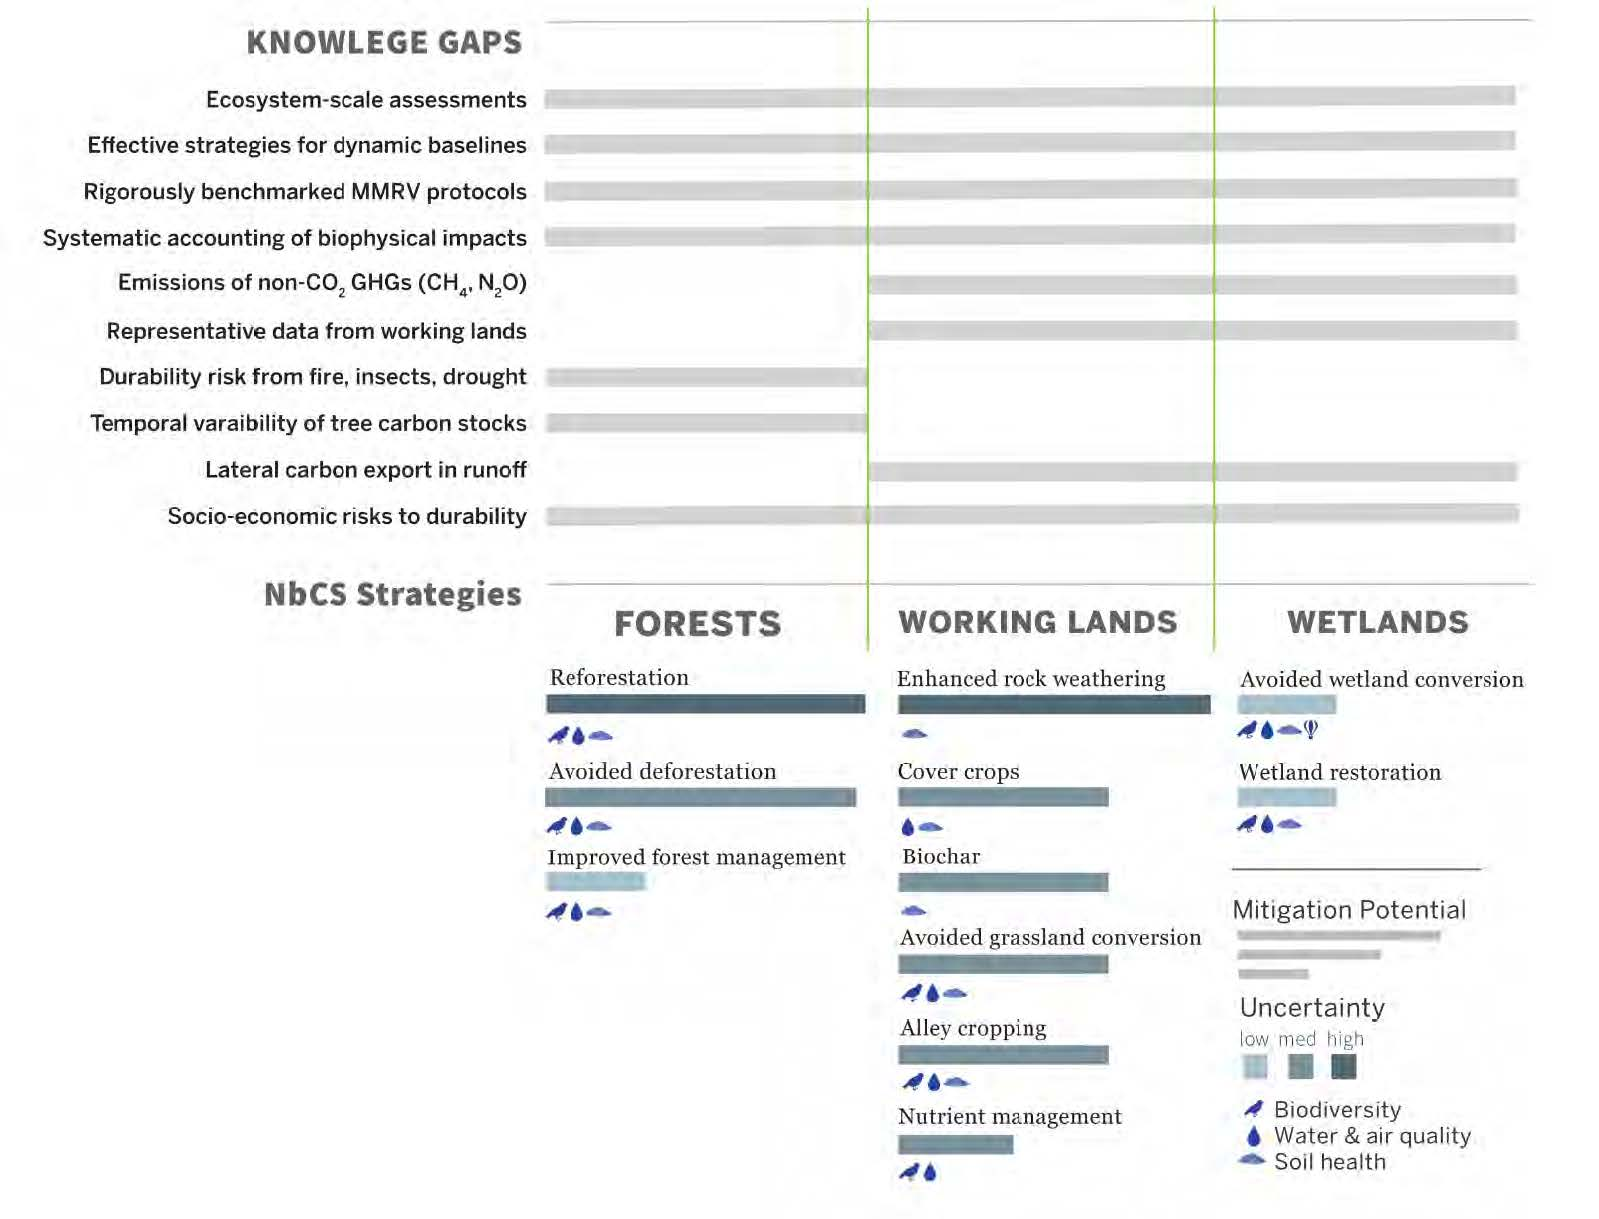
\includegraphics{img/01-nature-climate-solutions.jpg}

}

\caption{\label{fig-terrestrial-nature-solutions}In the bottom of the
figure, the length of the bar indicates (qualitatively) the expected
carbon mitigation potential, and the color represents uncertainty around
this potential. Icons indicating relevant co-benefits. Based largely on
information presented in Farigone et al.~201829. The top of the figure
highlights some of the most pressing knowledge gaps (see
Chapter~\ref{sec-overview} for more detail).}

\end{figure}

\hypertarget{key-criteria-limitations-and-opportunities}{%
\section{Key criteria, limitations, and
opportunities}\label{key-criteria-limitations-and-opportunities}}

While there is ample justification for implementing NbCS based on their
co-benefits alone, for NbCS to succeed specifically as climate
mitigation tools, they must meet four essential criteria:

\begin{itemize}
\tightlist
\item
  Criteria 1: Lead to enhancements to carbon uptake and/or reductions of
  non-CO2 GHGs that are additional to what would have occurred in a
  baseline or counterfactual scenario, and that integrate over all
  ecosystem sources and sinks.
\item
  Criteria 2: Lead to net cooling such that the biophysical effects on
  water and energy cycling do not overwhelm the gains in carbon uptake
  or emissions reductions.
\item
  Criteria 3: Achieve durable carbon storage by accounting for social
  and environmental risks to the permanence of ecosystem carbon storage
  and avoided GHG emissions.
\item
  Criteria 4: Account for leakage so that gains in one area are not
  canceled out by shifting activities to another area.
\end{itemize}

As discussed in detail in this report and elsewhere, major knowledge
gaps and concerns surrounding current NbCS activities and protocols
limit the extent to which they fulfill these criteria8,10,30,52,63,64
(Fig. 1). At regional and continental scales most relevant to
policy-setting, estimates of the present-day mitigation potentials of
NbCS vary substantially from one study to the next.2-4 These potentials
are usually estimated as a change in the amount of carbon residing in
two slowly evolving carbon stocks: shallow soil and aboveground plant
biomass. A focus on these two pools alone cannot capture the
ecosystem-scale carbon impacts of NbCS and tells us little about
emissions of non-CO2 GHGs (criteria 1). Moreover, for many NbCS,
existing data on how these stocks change are sparse and unrepresentative
of naturally occurring environmental gradients, limiting the available
information necessary to inform baselines against which additionality
can be calculated (criteria 1). A focus on changes in carbon stocks also
does not capture ``biophysical'' impacts of NbCS that can have both
favorable and unintended direct effects on temperature and water cycling
(criteria 2). Furthermore, the durability of carbon stored in soils and
woody biomass (criteria 3), as well as the leakage potential (criteria
4) are difficult to quantify and are not robustly considered in NbCS
accounting schemes. Together, these uncertainties reveal critical
challenges that hinder quantification of NbCS impacts from local to
continental scales, now and into the future.

Fortunately, substantial opportunity exists to address this uncertainty
by harnessing state-of-the-art carbon cycle measurement and prediction
tools together with lessons learned from practical experience in
implementing NbCS on the ground. The dominant role of terrestrial
ecosystems in determining atmospheric CO2 concentrations has been known
for decades. Consequently, huge investments of material resources have
fostered the development of innovative measurement technologies,
analytical tools, and predictive models for quantifying ecosystem carbon
cycles (Fig. 2). By and large, these tools have historically been used
for basic research of ecological processes and to inform global-scale
predictions for the future land carbon sink; but so far, the vast
majority have not been widely leveraged for what they might tell us
about expected and realized benefits of NbCS. Likewise, novel approaches
for crediting and verifying the climate benefits of NbCS are
proliferating at a range of scales, though most have not yet been widely
deployed61,62. Thus, right now, as we face a sea change in federal and
private-sector engagement with NbCS, we have a unique opportunity to
integrate the best-available science into next-generation information
systems to support effective NbCS programs and policy that address all
four key criteria.

\begin{tcolorbox}[enhanced jigsaw, coltitle=black, rightrule=.15mm, titlerule=0mm, opacitybacktitle=0.6, leftrule=.75mm, toprule=.15mm, arc=.35mm, breakable, colback=white, left=2mm, colbacktitle=quarto-callout-note-color!10!white, colframe=quarto-callout-note-color-frame, toptitle=1mm, title=\textcolor{quarto-callout-note-color}{\faInfo}\hspace{0.5em}{Box 1: Elements of robust, scalable, and credible NbCS}, bottomtitle=1mm, opacityback=0, bottomrule=.15mm]

\begin{itemize}
\tightlist
\item
  \textbf{Robust:} NbCS incentivization programs fully address all four
  key criteria (additional mitigation, net cooling, durability, and
  leakage). Doing so means that NbCS accounting schemes

  \begin{enumerate}
  \def\labelenumi{\arabic{enumi}.}
  \tightlist
  \item
    are informed by ecosystem-scale data that integrate over all carbon
    sources and sinks,
  \item
    consider a full set of GHG fluxes,
  \item
    explicitly account for the durability of carbon stored in soils and
    tree biomass and the possibility of leakage, and
  \item
    are holistic, considering not only the climate mitigation potential,
    but also coupled biophysical impacts on energy and water cycling.
  \end{enumerate}
\item
  \textbf{Scalable:} The strategies used to quantify the benefits of
  individual NbCS projects are harmonized with approaches to map the
  same benefits over regional and continental scales, so that NbCS
  programs can be informed by an understanding of when and where
  specific strategies are most likely to succeed.
\item
  \textbf{Credible:} The policy instruments used to incentivize NbCS
  rely on monitoring and quantification tools that are rigorously
  standardized and cross-compared, with open and transparent data and
  code sharing, allowing for independent validation of all activities
  and projections.
\end{itemize}

\end{tcolorbox}

\hypertarget{a-path-forward}{%
\section{A path forward}\label{a-path-forward}}

The objective of this report, which is co-authored by experts in both
NbCS science and implementation, is to describe the technologies, tools
and approaches necessary to support robust, scalable, and credible NbCS
strategies for the US. The report is organized around the identification
of key knowledge gaps and pathways to close them, providing a road map
for actionable, cross-sectoral information to foster NbCS strategies
that work while avoiding energy wasted on NbCS strategies that have
limited environmental benefits or the potential to backfire and
exacerbate climate change. The criteria for robust, scalable, and
credible NbCS defined in Box 1.

Before we proceed, there are two things to keep in mind. First, it is
important to distinguish between the concepts of ``technical mitigation
potential'' and ``realizable mitigation potential,'' which is sometimes
also referred to as ``social potential'' or ``economic potential.''
Technical mitigation potential describes increases in carbon uptake
and/or reductions in GHGs emissions that are theoretically achievable
through NbCS interventions, usually determined per unit area and summed
across all available areas. The factors that influence the technical
potential include heterogeneity in biophysical factors like climate,
species composition, and nutrient cycles, as well as uncertainties in
our ability to accurately measure changes in fluxes of CO2 and other
GHGs. The realizable mitigation potential includes other factors, such
as the sociological and economic forces that determine landowner
willingness to adopt or sustain a ``climate-smart'' practice. This
report is most strongly focused on research needed to quantify and
predict the technical mitigation potential of NbCS. Frequently, gaps and
research needs related to the realizable potential are also highlighted.

Second, the knowledge gaps that we identify in Section 2 are not trivial
and appear to reveal a wide gulf between the state-of-the-science
surrounding NbCS and the pace at which NbCS strategies are being
implemented on the ground. Indeed, there are many points of disconnect,
including a lack of consensus among scientists about the realizable
climate benefits of these strategies56, a dearth of representative data
necessary for more confident quantification of NbCS impacts, and the
fact that many protocols used for most NbCS project accounting were
developed decades ago and do not leverage the best-available science.
However, it is important to remember that terrestrial ecosystem ecology
is a well-established field of study, and over the decades, we have
gained a tremendous amount of knowledge about the mechanisms that drive
variability in ecosystem carbon, water, energy, and nutrient cycles.
Critically, we have also developed a wide variety of pre-existing
experimental sites, datasets, technologies, and analytical tools that
have not yet been fully leveraged for what they reveal about NbCS (see
Section 3). Thus, relatively subtle shifts in the research questions we
ask and the scale at which we ask them, combined with strategic
expansion of existing field sites and monitoring networks, could
substantially alleviate the burden of material resource investment
necessary to address these knowledge gaps (see details in Section 4).

\begin{figure}

{\centering 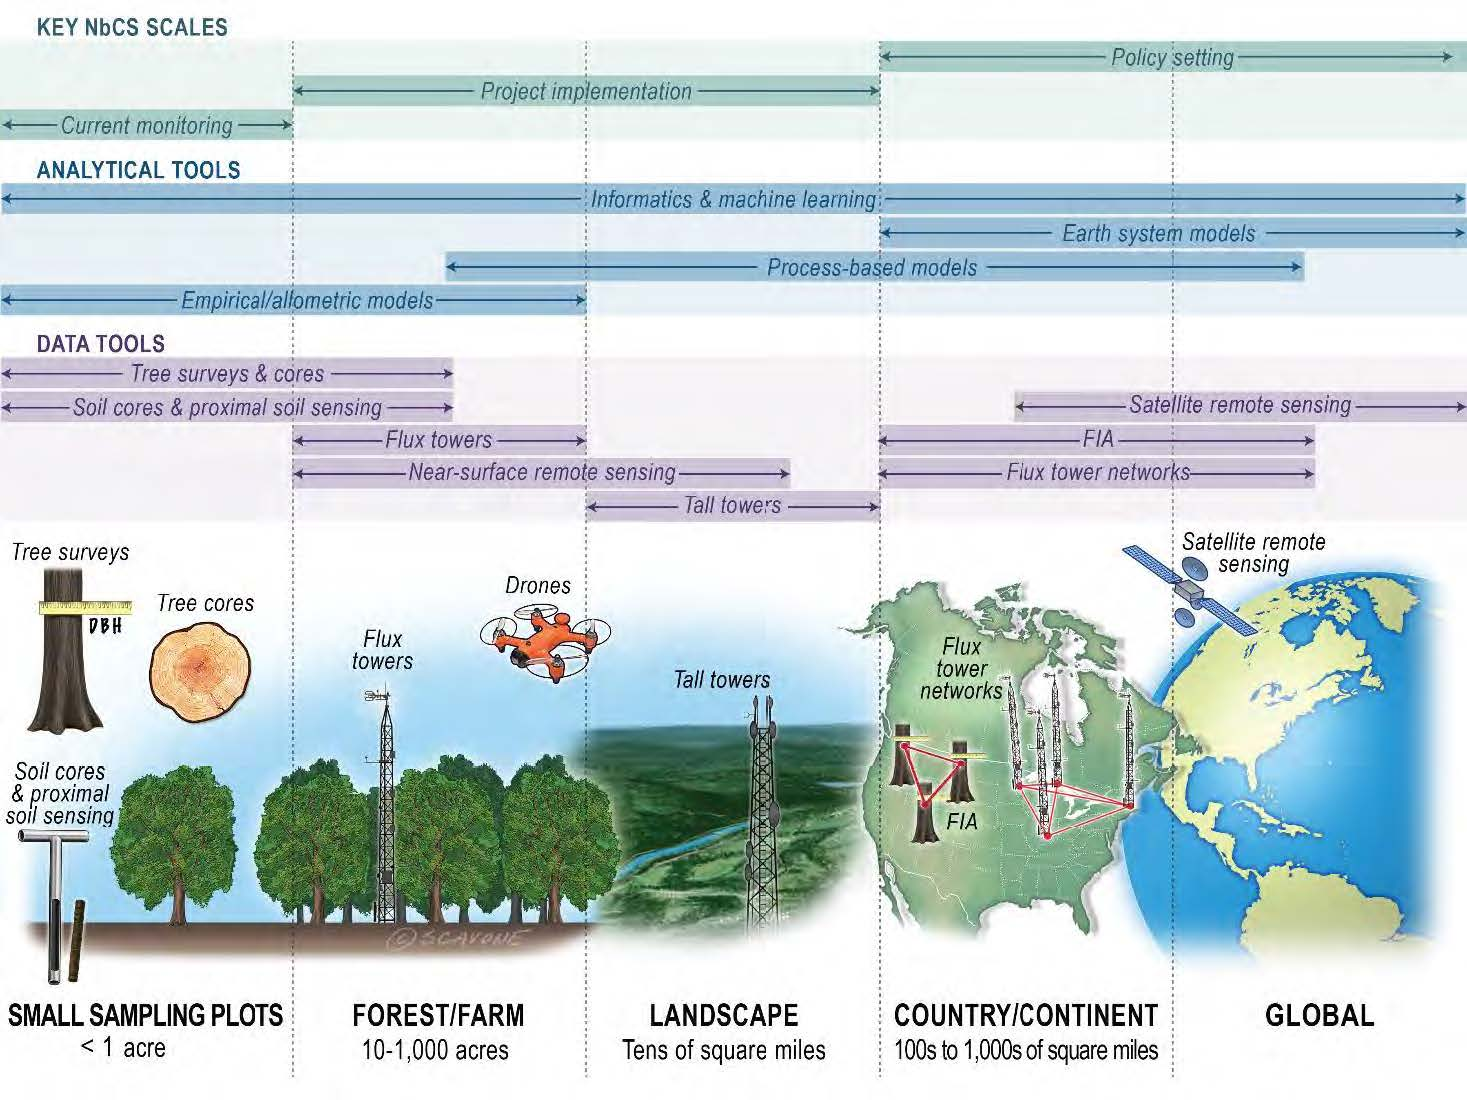
\includegraphics{img/02-nbcs-scales.jpg}

}

\caption{\label{fig-ncbsscales}The data and analytical tools that could
be more fully leveraged to inform NbCS. See Section 3 for details. Image
copyright William Scavone. All rights reserved.}

\end{figure}

\bookmarksetup{startatroot}

\hypertarget{sec-knowledge}{%
\chapter{Knowledge Gaps Limiting Robust, Scalable and Credible NbCS for
the United States}\label{sec-knowledge}}

\hypertarget{knowledge-gaps-related-to-field-data-scarcity}{%
\section{Knowledge gaps related to field data
scarcity}\label{knowledge-gaps-related-to-field-data-scarcity}}

Our understanding of the technical mitigation potential of many NbCS
strategies is limited by a scarcity of representative field data, either
because these data do not yet exist or because they are not yet freely
accessible. Notable exceptions exist, including networks of
ecosystem-scale flux towers (e.g., AmeriFlux65,66 and NSF's National
Ecological Observatory Network, or NEON67) and the wealth of information
on tree biomass and associated stand dynamics supported by the USDA
Forest Service Forest Inventory and Analysis (FIA) program68. These
networks may provide sufficiently representative data to map carbon
fluxes at coarse scales69, or even to estimate potential changes in
plant carbon stocks achievable with some NbCS like reforestation70,71.
However, networks like NEON, FIA and AmeriFlux were not designed
specifically with the goal of evaluating NbCS, and many specific NbCS
management strategies (e.g., cover crops, soil amendments, altered
forest management, wetland restoration) are potentially un- or
under-represented in these networks. These networks were also not
designed to be interoperable, which makes it difficult to blend
information from disparate networks (e.g., FIA and AmeriFlux) into
synthetic analyses and products. Efforts to dynamically catalog existing
NbCS field trials and the activities of relevant monitoring networks
would permit an informed prioritization of new data collection and
facilitate synthesis of new and existing network data.

\bookmarksetup{startatroot}

\hypertarget{references}{%
\chapter*{References}\label{references}}
\addcontentsline{toc}{chapter}{References}

\markboth{References}{References}

\hypertarget{refs}{}
\begin{CSLReferences}{1}{0}
\leavevmode\vadjust pre{\hypertarget{ref-novick-et-al22}{}}%
Novick, Kim, Christopher Williams, Benjamin Runkle, William Anderegg,
Dave Hollinger, and Marcy Litvak. 2022. {``The Science Needed for
Robust, Scalable, and Credible Nature-Based Climate Solutions for the
United States: Full Report.''} Bloomington: Indiana University Libraries
Department of Scholarly Communication.
\url{https://doi.org/10.5967/n7r9-7j83}.

\leavevmode\vadjust pre{\hypertarget{ref-walker-et-al19}{}}%
Walker, Xanthe J., Jennifer L. Baltzer, Steven G. Cumming, Nicola J.
Day, and Christopher Ebert. 2019. {``Increasing Wildfires Threaten
Historic Carbon Sink of Boreal Forest Soils.''} \emph{Nature}, no. 572.

\end{CSLReferences}



\end{document}
